\section{Procedure and results}
Besides the experiemntell procedure, this section presents as main results the
absorption spectrum of Rubidium. Therefore, the setup shown in figure \ref{fig: setup}
is used. Before an examination of the spectrum is possible, the laser system has to be
adjust correctly.

To operate the laser properly, the diode must be heated
continuously to $\SI{50}{\degreeCelsius}$. During the heating process, a infrared display
card is inserted in the path of the later laser beam. After the diode reached
the target temperature, the diode current ist increased slowly until a
light spot is visible on the display card. Depending on the current are
two emission modes of the laser observerable as presented in figure \ref{fig: emission_modes}.
\begin{figure}
  \centering
      \begin{subfigure}{0.48\textwidth}
          \centering
          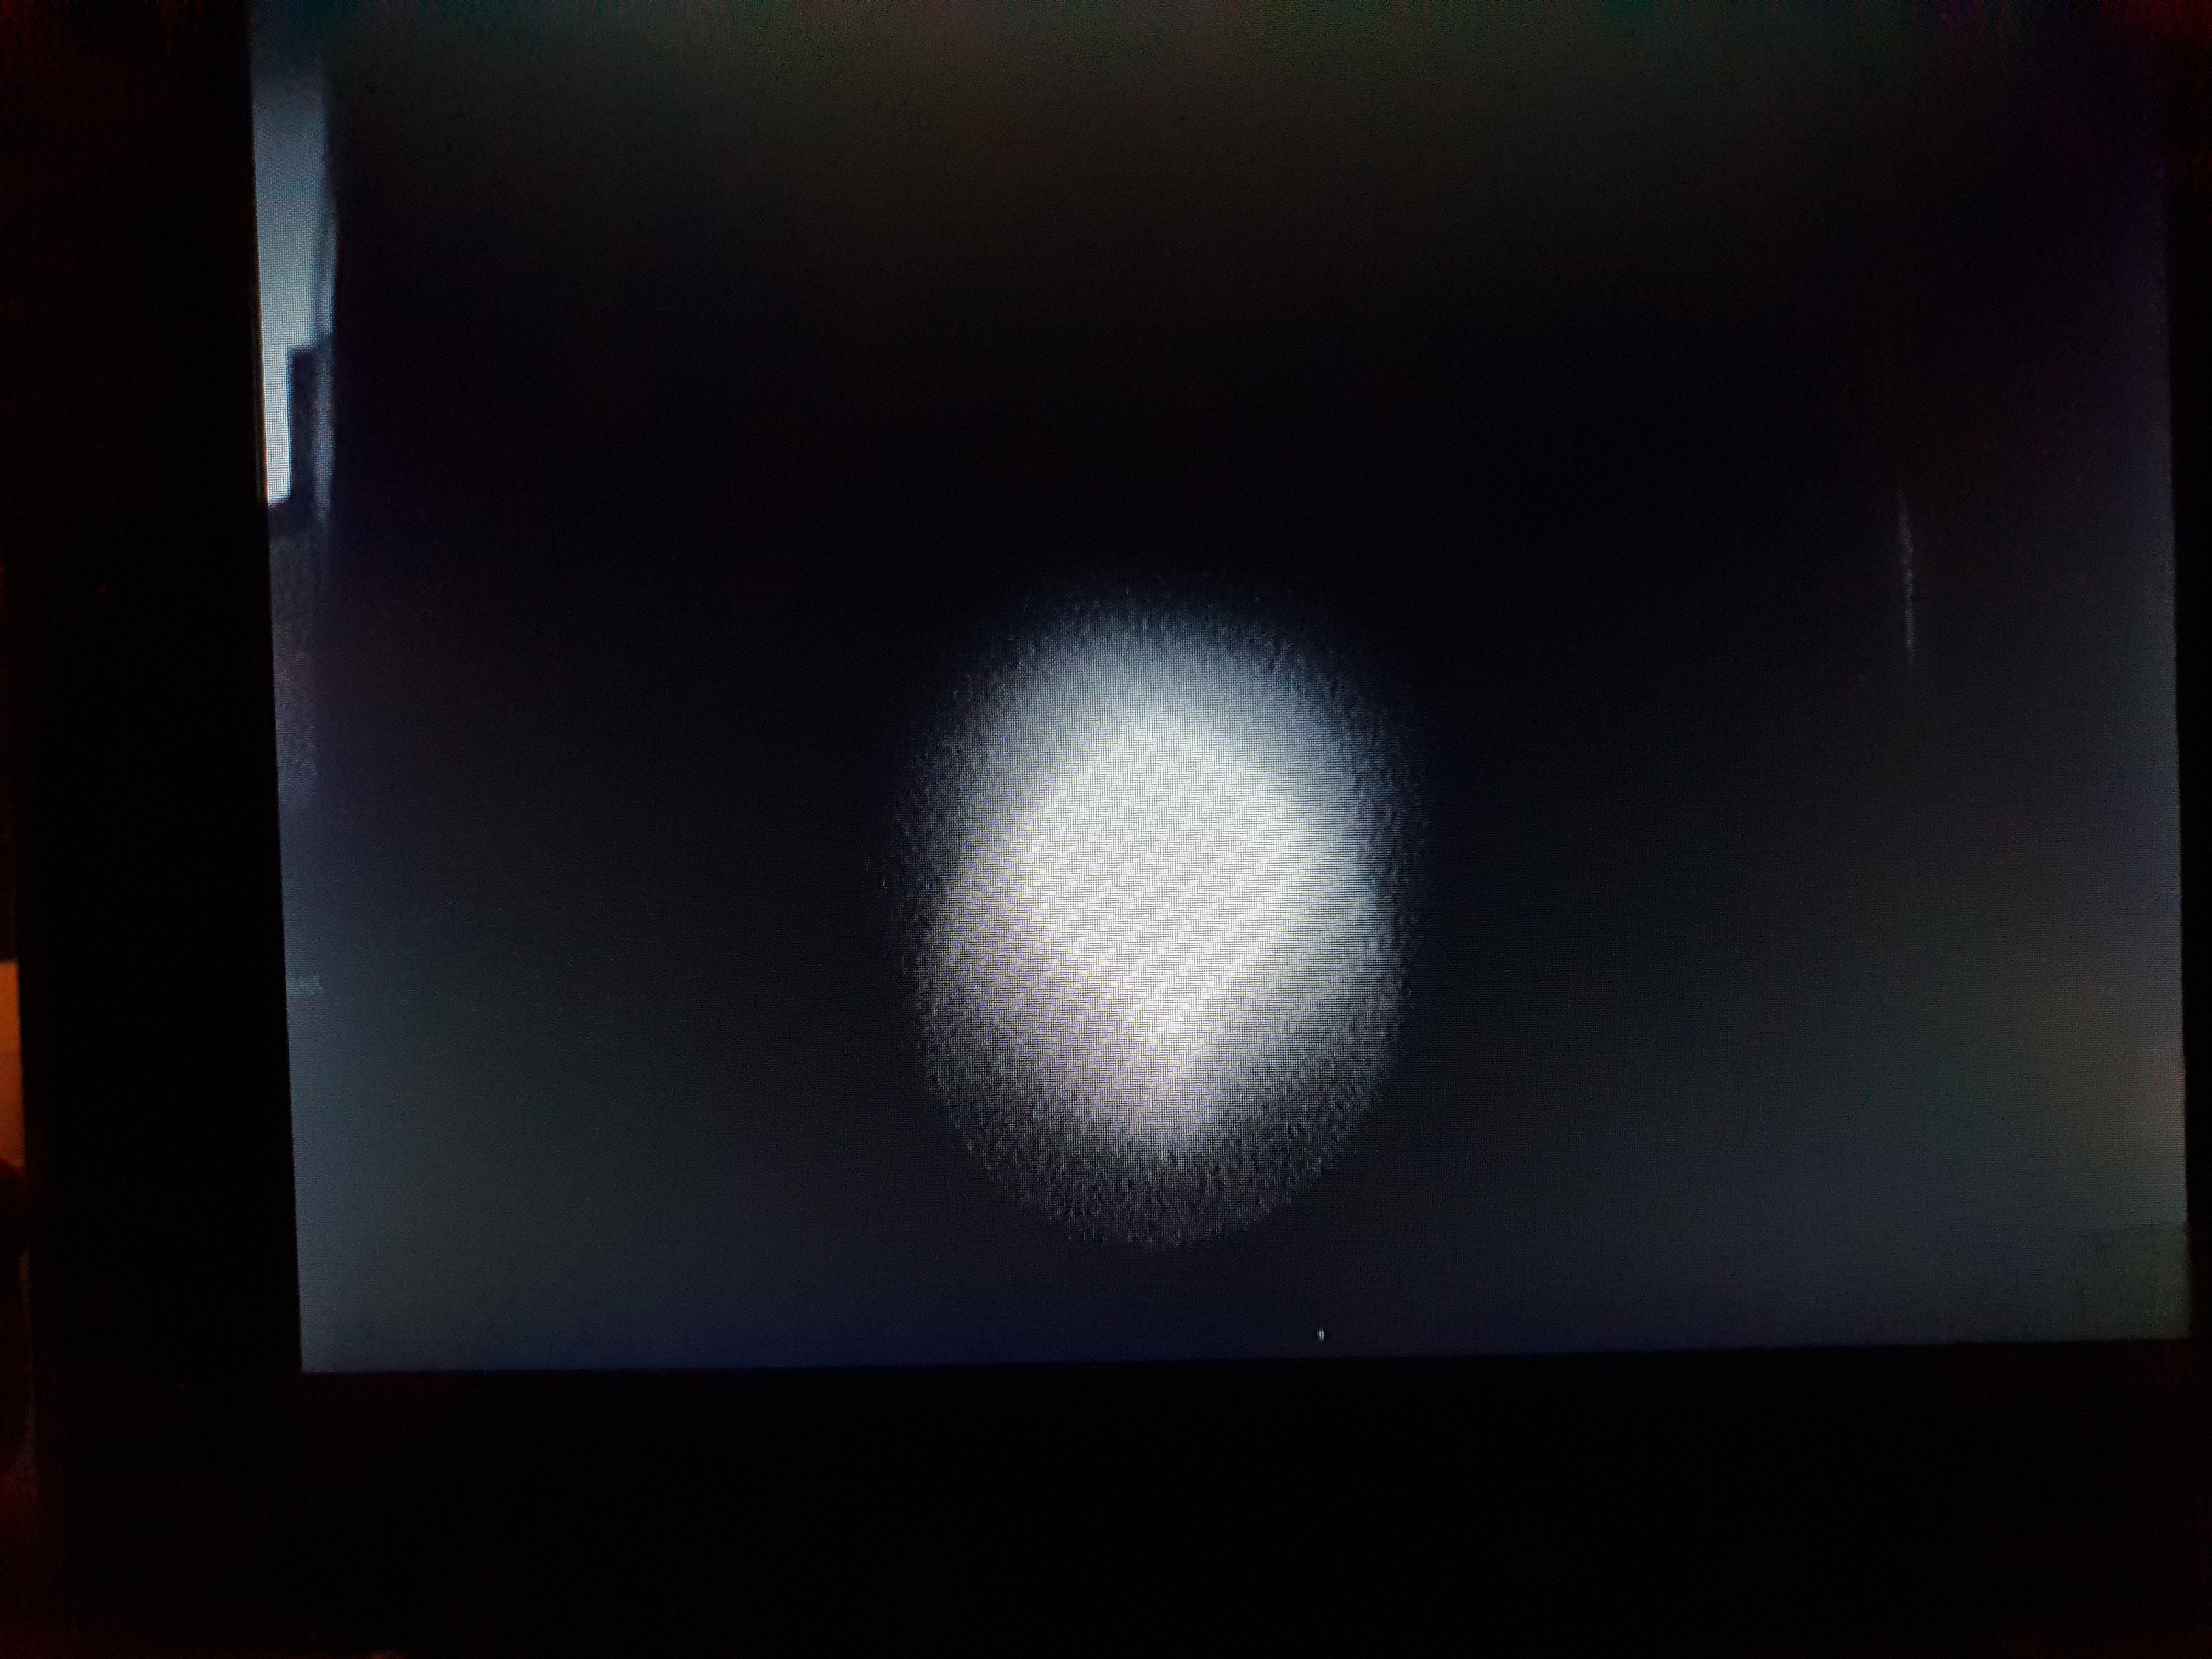
\includegraphics[width = \textwidth]{./content/images/diodelaser_not_lasering.jpg}
          \caption{Not lasering.}
          \label{fig:not_lasering}
      \end{subfigure}
      \begin{subfigure}{0.48\textwidth}
          \centering
          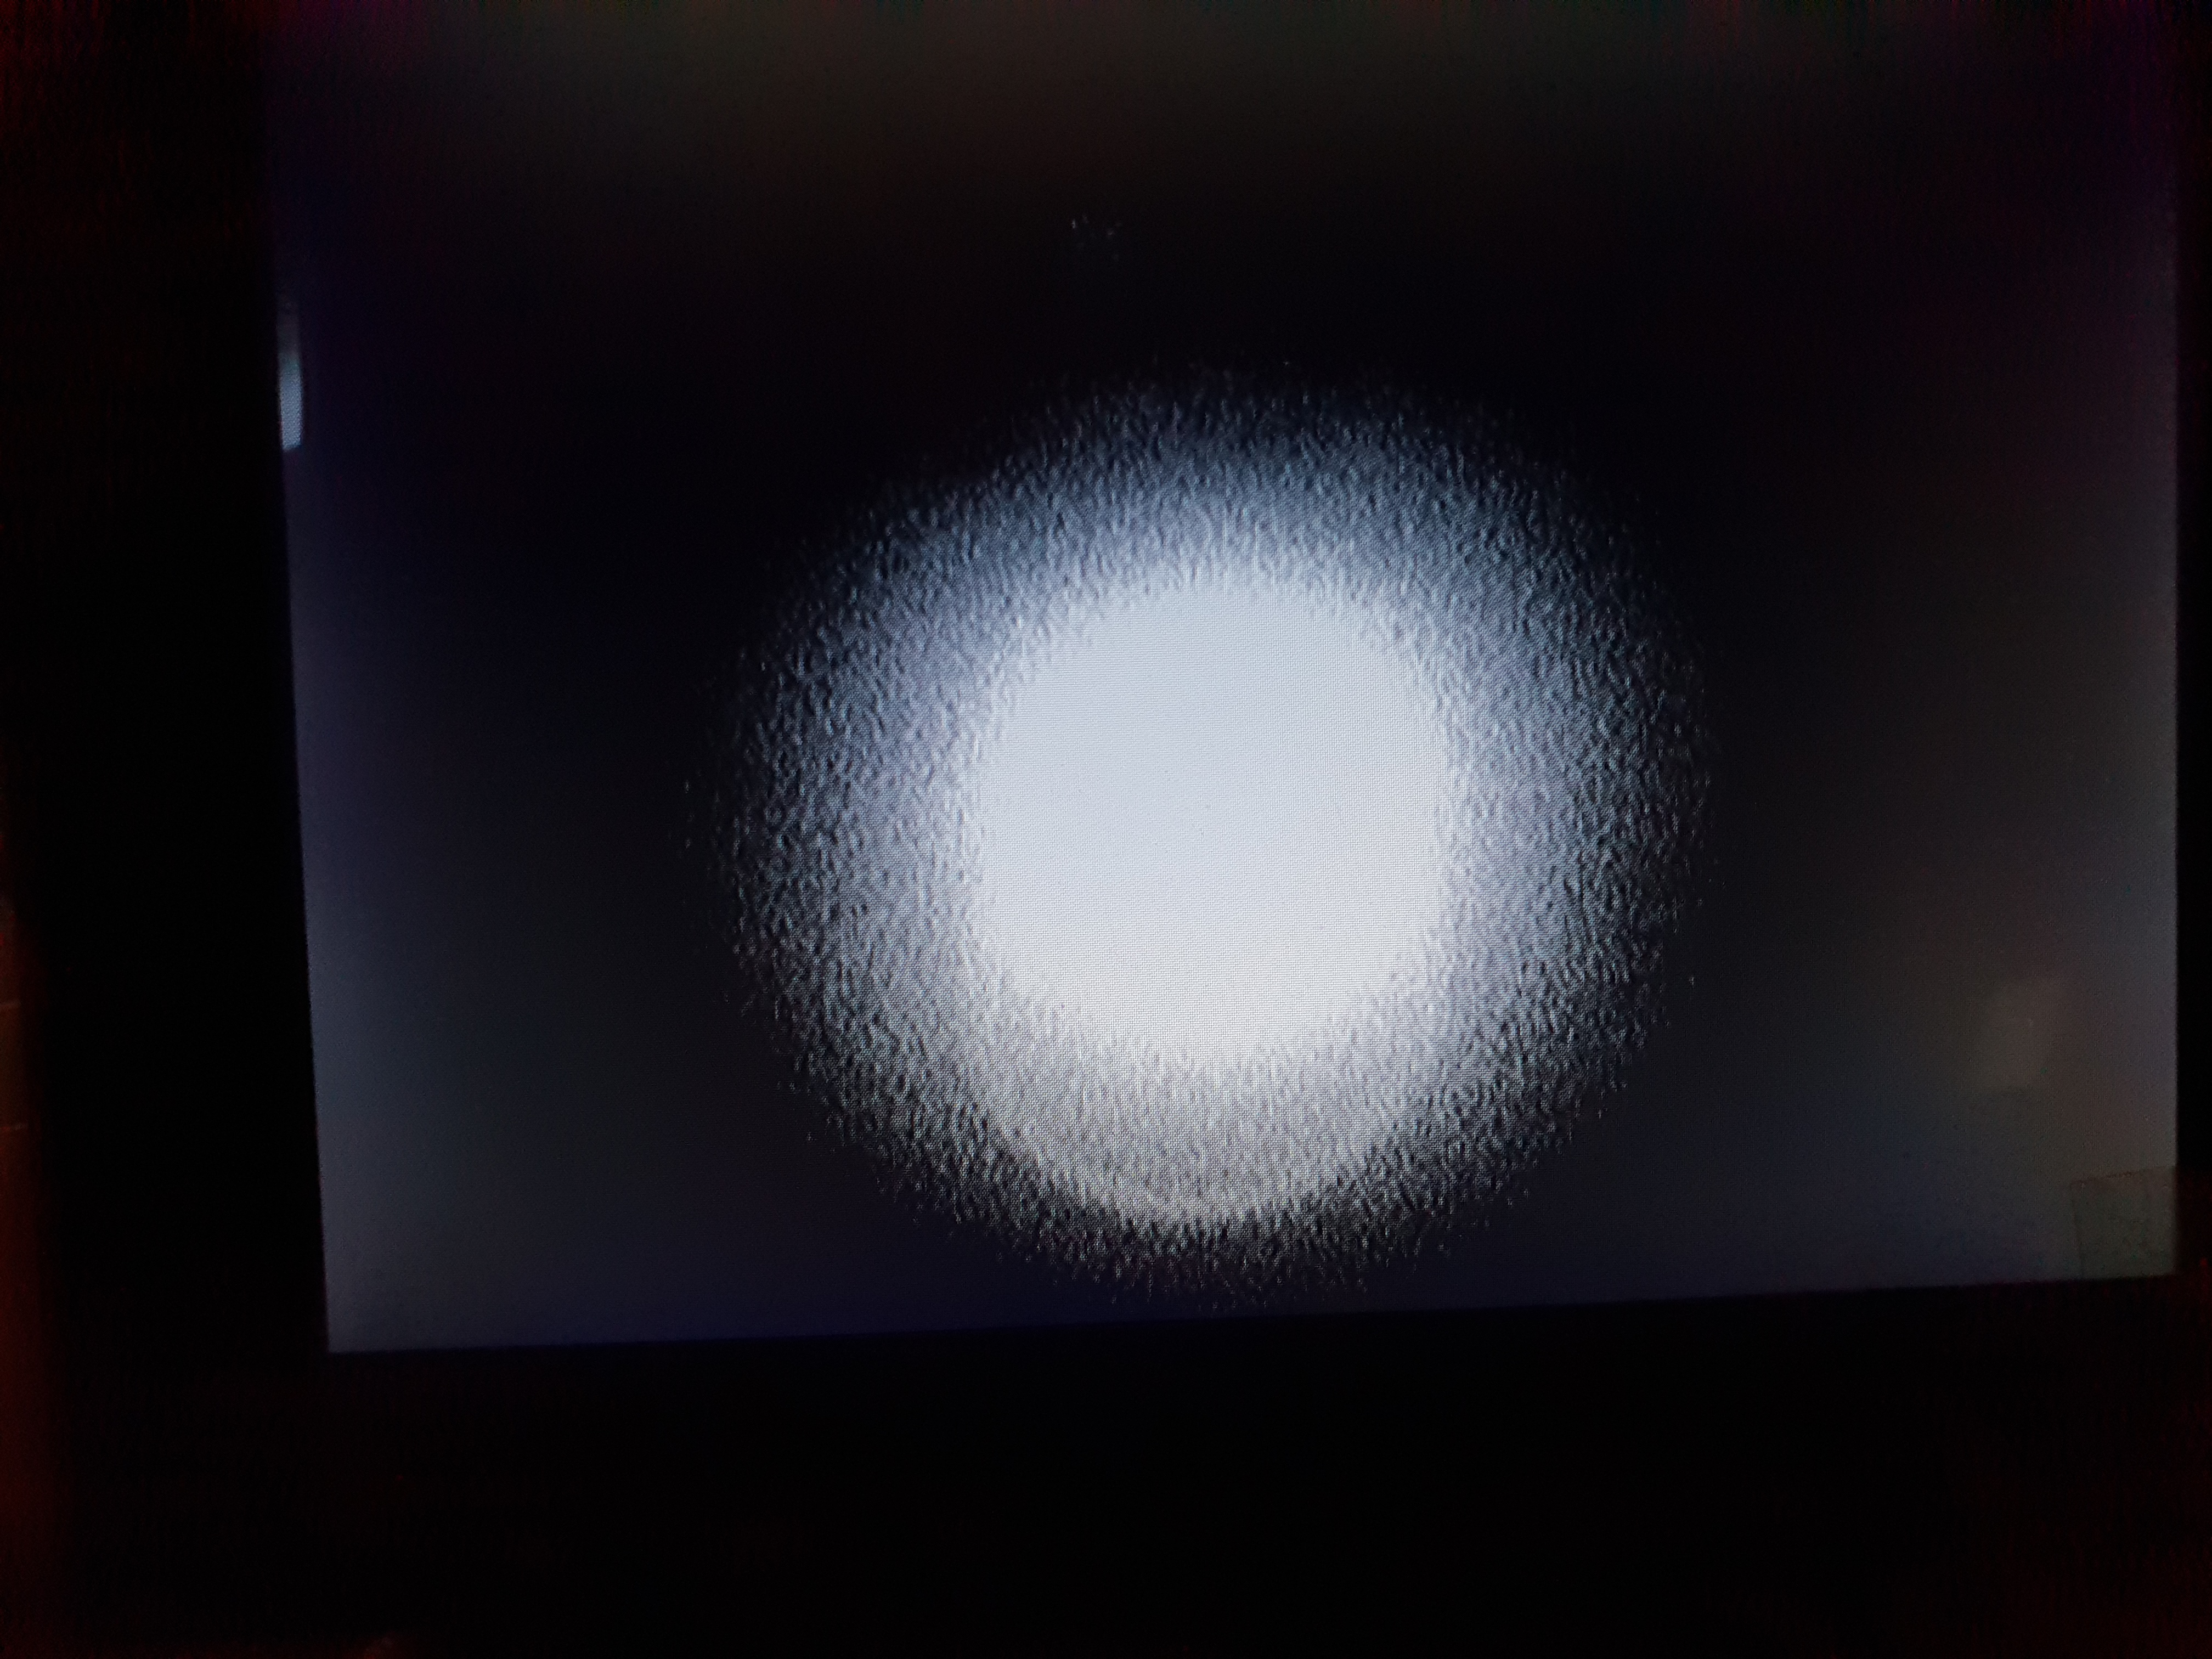
\includegraphics[width = \textwidth]{./content/images/diodelaser_lasering.jpg}
          \caption{Lasering.}
          \label{fig:lasering}
      \end{subfigure}
  \caption{Observerd emission modes of the laser. The diode laser behaves like a regular
  LED under a certain current threshold, \ref{fig:not_lasering}. After reaching the
  current threshold the diode laser emits coherent light \ref{fig:lasering}. }
\label{fig: emission_modes}
\end{figure}
If the current reaches a certain threshold, the diode starts to emit coherent
light, and can be used as laser. To operate the diode laser efficently,
the current is decreased slightly below the threshold. The light spot on the
diplay card is now equal to image \ref{fig:not_lasering}. By moving the knobs
on the diffraction grating carefully, the diode starts to emit coherent light
as shown in image \ref{fig:lasering}. The knobs slightly changes the length of
the external cavity and how the light reflected from the grating hits the diode.
